\section{Lecture 7: Waves, water dynamics and tides}

\subsection{How are waves formed?}

\begin{itemize}
    \item Waves are created by energy release including:
    \begin{itemize}
        \item Wind
        \item Movement of media (air or fluids) of different densities:
        \begin{itemize}
            \item Air-water = ocean waves
            \item Air-air = atmospheric waves
            \item Water-water = internal waves
        \end{itemize}
        \item Mass movement into the ocean (splash waves, but also commonly grouped
            into the category of tsunamis)
        \item Underwater seafloor movement (tsunami)
        \item Pull of the Moon and Sun (tides)
        \item Atmospheric pressure changes (seiches)
        \item Human activities (explosions)
    \end{itemize}
    \item Progressive waves move energy, not mass!
\end{itemize}

\subsection{Internal waves}

Pycnocline = a layer in a body of water where the density changes rapidly with depth,
typically separating warmer, less dense surface water from colder, denser deep water.

\subsection{Most ocean waves are wind-generated}

\subsection{Types of progressive waves}

Progressive waves oscillate uniformly and travel without breaking.

\begin{enumerate}
    \item Longitudinal (compressional): back-and-forth particle motion in solid,
        liquid and gas
    \item Transverse (shear): side-to-side particle motion in solids only (not in ocean)
    \item Orbital (e.g. typical wind waves): combination of longitudinal
        and transverse in liquids and/or gas
\end{enumerate}

\subsection{Wave characteristics and terminology}

\begin{itemize}
    \item Crest
    \item Trough
    \item Wave height (H)
    \item Wavelength (L)
    \item Still water level
    \item Orbital motion
    \item Wave base
\end{itemize}

\begin{figure}[H]
    \centering
    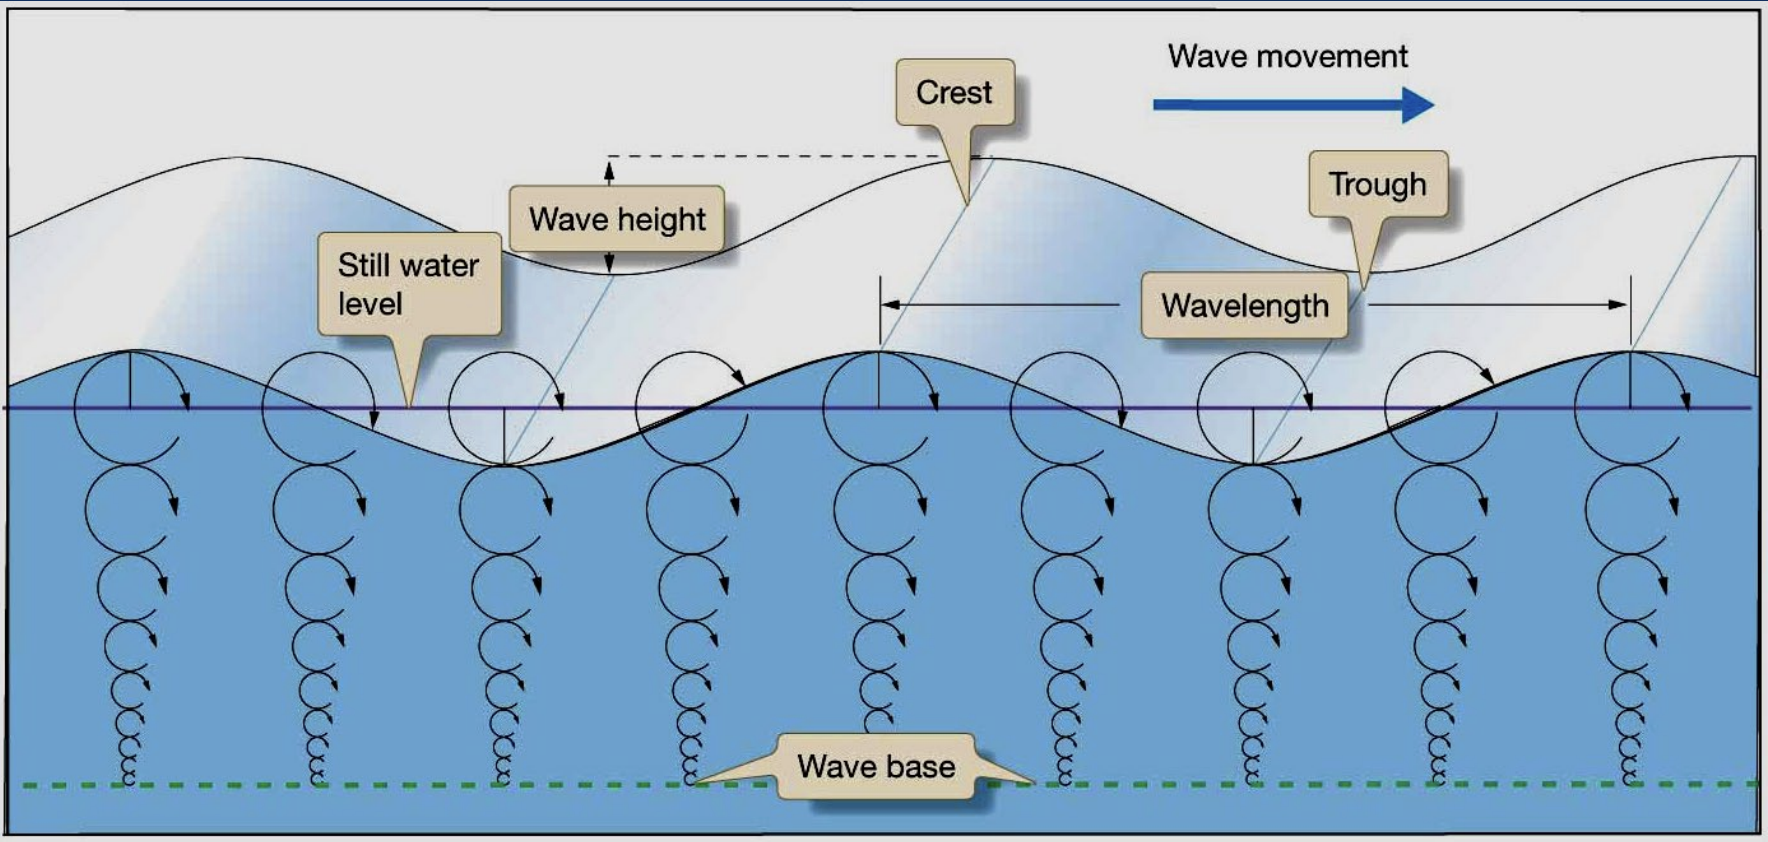
\includegraphics[width=0.9\linewidth]{img/wave_characteristics.png}
\end{figure}

\begin{figure}[H]
    \centering
    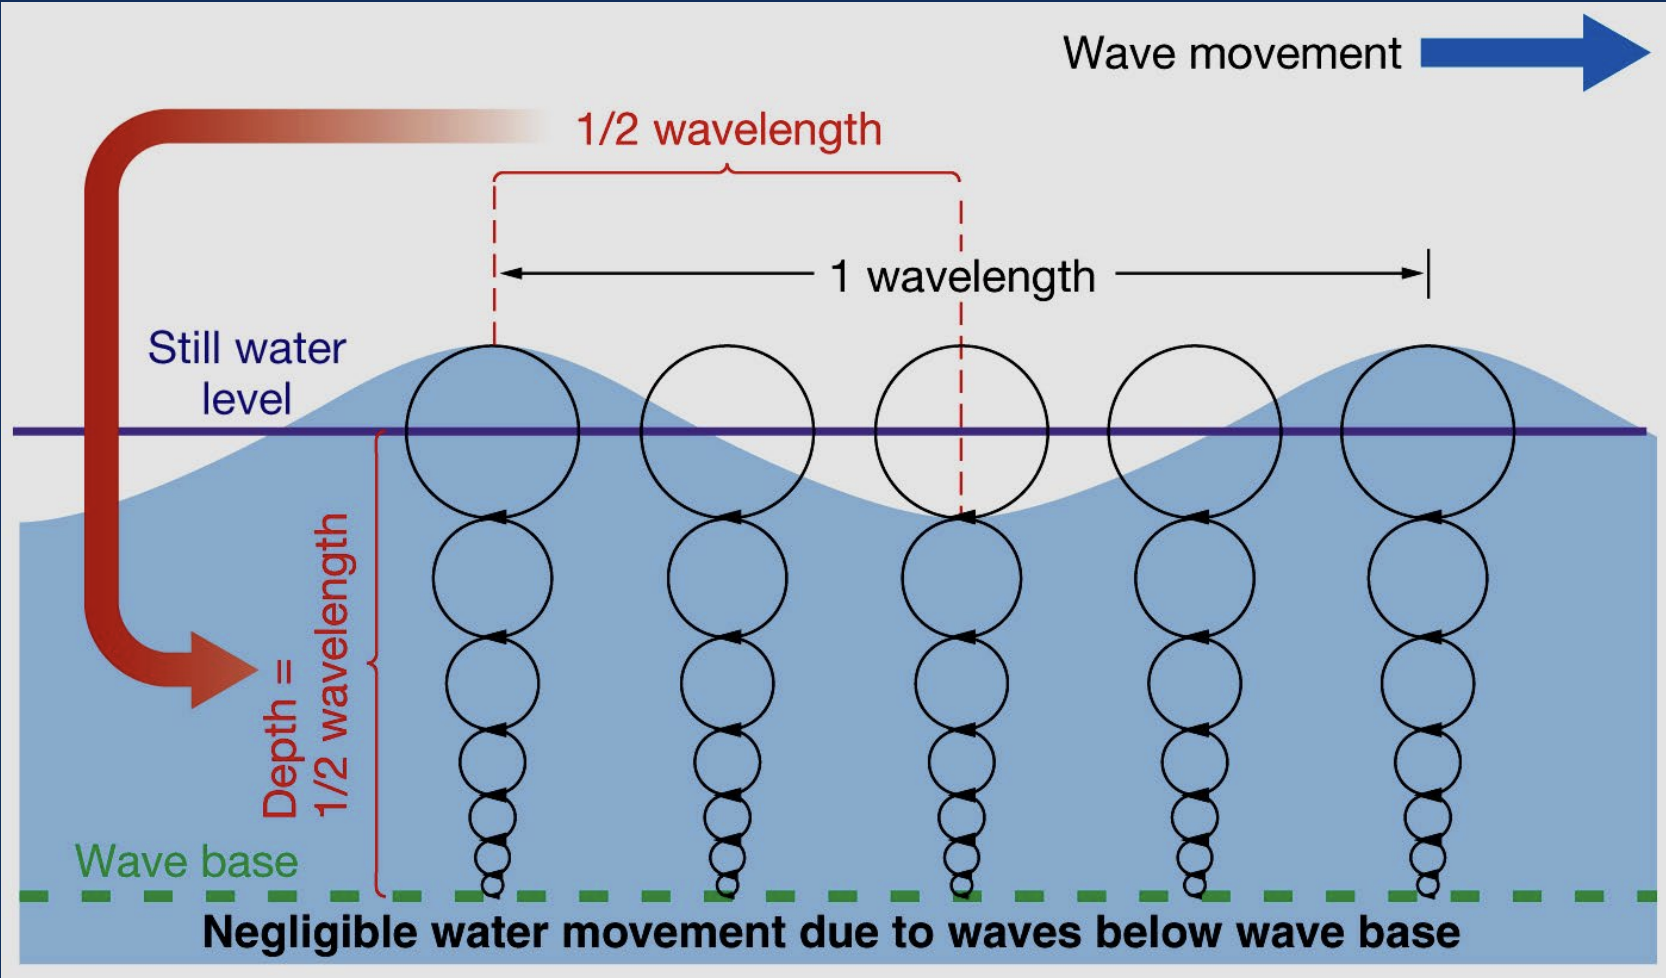
\includegraphics[width=0.9\linewidth]{img/wave_characteristics2.png}
\end{figure}

\begin{itemize}
    \item Orbital size decreases with depth to zero at the wave base
    \item Depth of wave base = one half wavelength (L/2), measured
        from still water level
\end{itemize}

\subsection{Wind waves and how they break when reaching the coasts}

\subsection{Wind driven wave}

\subsection{Waves undergo physical changes in the surf zone}

\begin{itemize}
    \item As swell moves towards the coast, the water depth decreases,
        and at water depth of half the wavelength, the wave energy touches
        the seafloor, and energy will eventually be released by breaking waves.
    \item As the base of the wave touches the seafloor, the wave speed decreases.
    \item The wave behind is still traveling at the same speed as before,
        so the wavelength decreases.
    \item Some energy is lost to friction, but the remaining energy must go somewhere,
        so the wave height increases.
    \item When the wave steepness (H/L) > 1/7, breakers form and energy is released in the
        surf zone.
\end{itemize}

\begin{figure}[H]
    \centering
    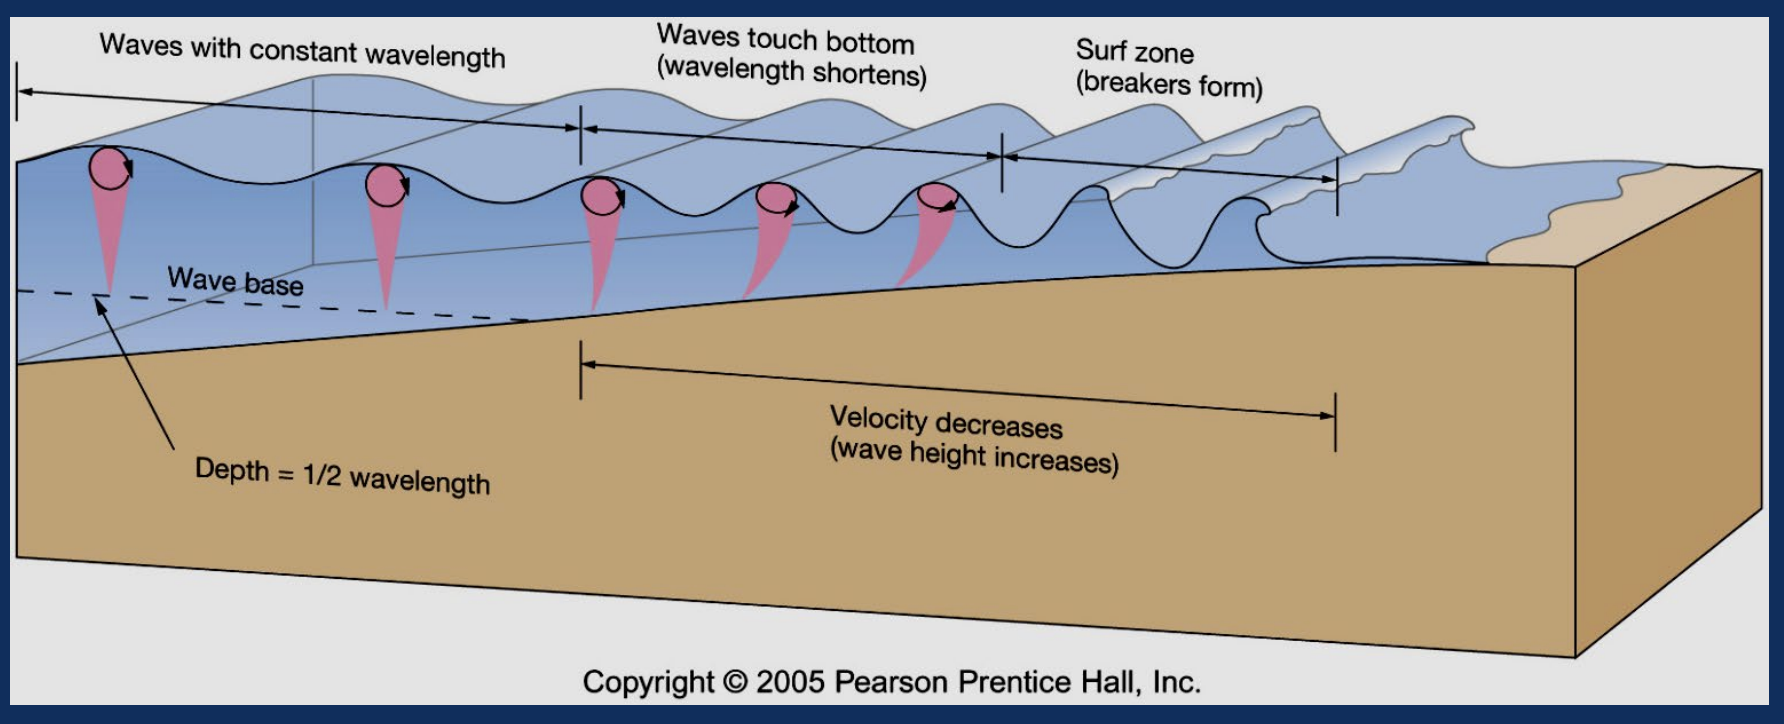
\includegraphics[width=0.9\linewidth]{img/wave_surf_zone.png}
\end{figure}

\subsection{Wave interference patterns}

\begin{itemize}
    \item Constructive interference: troughs and crests aligned between
        two waves; increases wave height.
    \item Destructive interference: troughs of one wave lined up
        with crests of another wave; decreases wave height.
    \item Mixed: variable pattern.
\end{itemize}

\subsection{Tsunamis}

\begin{itemize}
    \item Tsunami terminology:
        \begin{itemize}
            \item Often called "tidal waves" but have nothing
                to do with the tides
            \item Japanese term meaning "harbor wave"
            \item Also called "seismic sea waves"
        \end{itemize}
    \item Created by movement of the ocean floor by:
        \begin{itemize}
            \item Underwater fault movement
            \item Underwater slides
            \item Underwater volcanic eruptions
        \end{itemize}
\end{itemize}

Most tsunami originate from underwater fault movement.

\begin{figure}
    \centering
    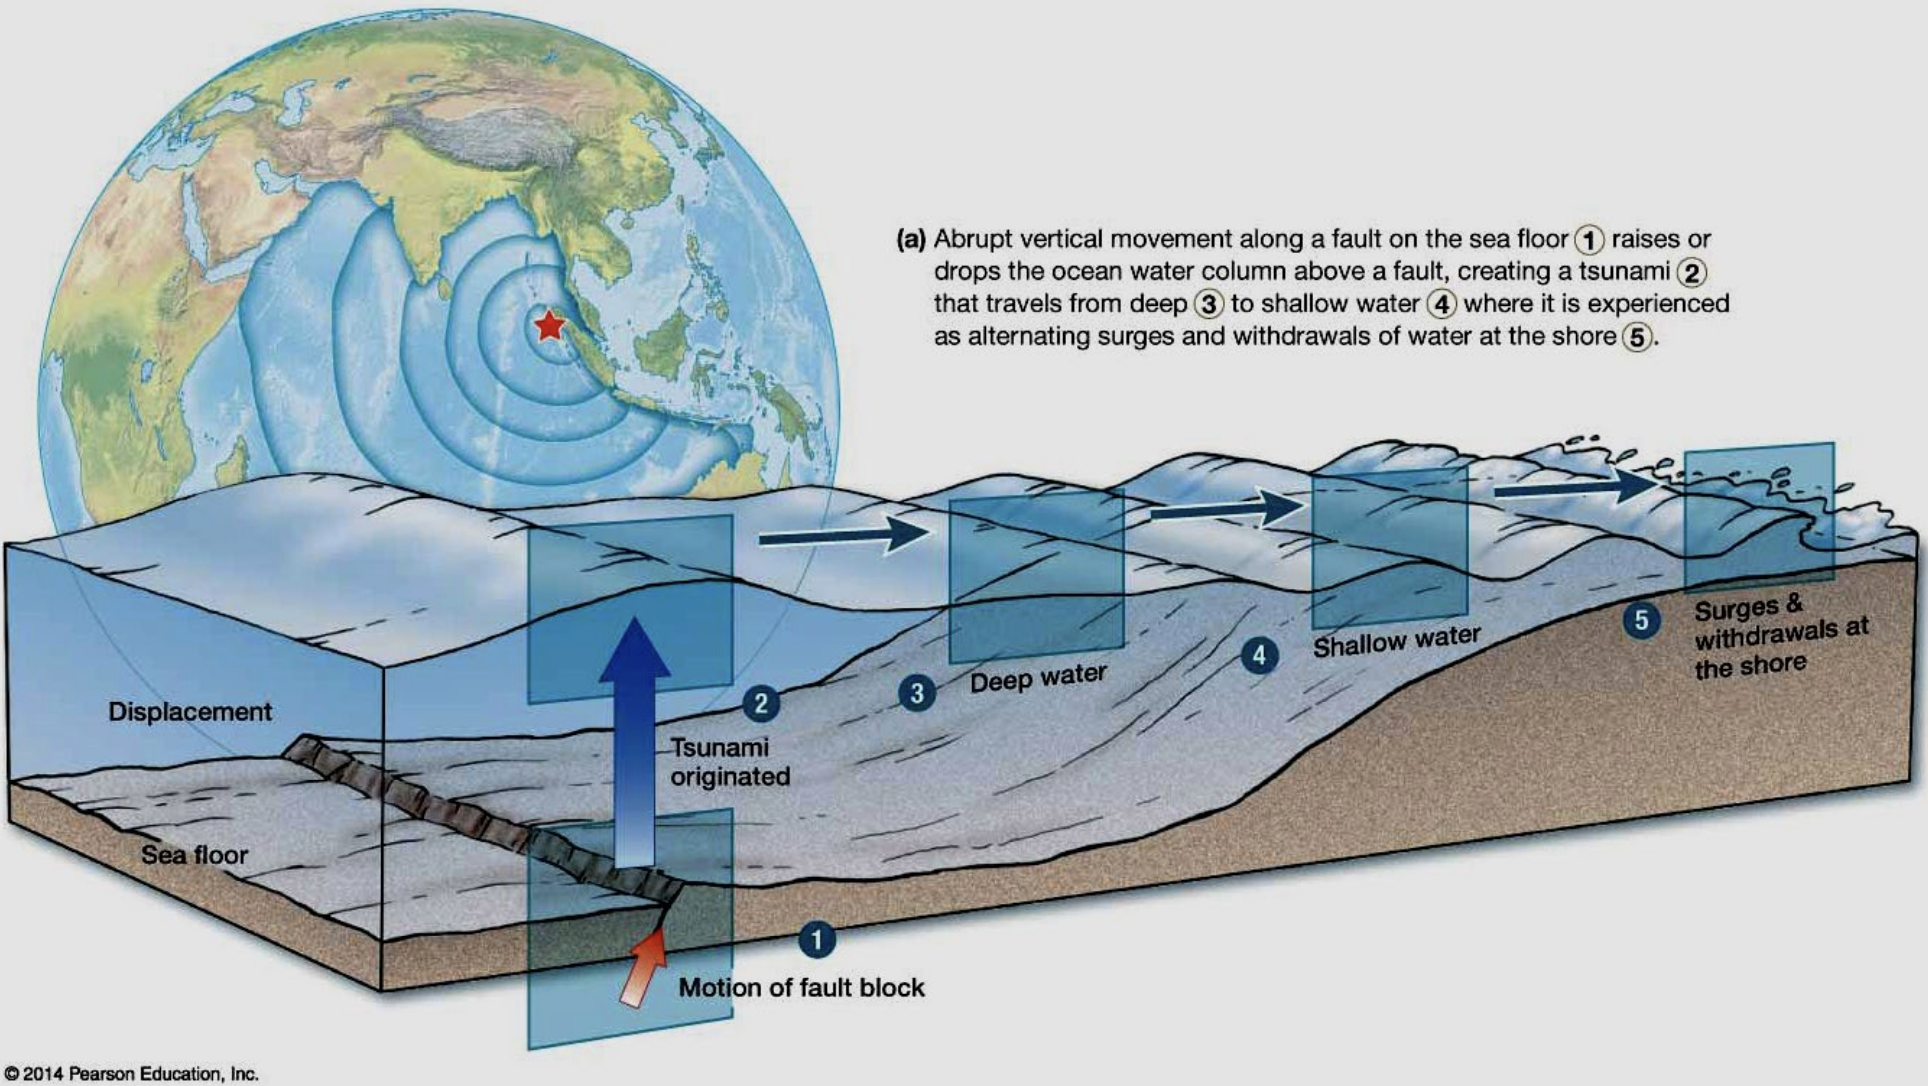
\includegraphics[width=0.75\linewidth]{img/tsunami.png}
\end{figure}

\subsection{Costal effects of tsunami}

\begin{itemize}
    \item If a trough arrives first, it appears as a strong
        withdrawal of water (similar to an extreme and suddenly-occurring
        low tide)
    \item If a crest arrives first, it appears as a strong surge of water
        that can raise sea level many meters and flood inland areas
    \item Tsunami often occur as a series of surges and withdrawals over hours
\end{itemize}

\subsection{What are tides?}

\begin{itemize}
    \item Tides are the daily periodic raising and lowering of sea level.
    \item Tides are very long and regular shallow water waves.
\end{itemize}

\subsection{What causes tides?}

\begin{itemize}
    \item Gravity
    \begin{enumerate}
        \item Gravitational force of the Moon and Sun on Earth
        \begin{itemize}
            \item If mass increases, then gravitational force increases
            \item If distance increases, then gravitational force greatly
                decreases
        \end{itemize}
        \item Centripetal (center-seeking) gravity force required to keep
            planets/moon/sun in nearly circular orbits around each other
    \end{enumerate}
\end{itemize}
